\subsection{Multivariate meta-analysis}
A related situation arises in random effects multivariate
meta-analysis
\citep{Berkey-etal:1998,Nam-etal:2003},
where several outcome measures are observed in a series of
similar research studies and it is desired to synthesize
those studies to provide an overall (pooled) summary of the outcomes
together with meta-analytic inferences and
measures of heterogeneity across studies.

The application of mixed model ideas in this context differs
from the standard situation in that individual data are
usually unavailable and use is made instead of
summary data (estimated treatment effects and their covariances)
from the published literature. The multivariate extension of standard
univariate methods of meta-analysis allows the correlations among
outcome effects to be taken into account and estimated, and
regression versions can incorporate study-specific covariates to
account for some inter-study heterogeneity. More importantly,
we illustrate a graphical method based (of course) on ellipsoids
that serves to illustrate bias, heterogeneity, and shrinkage in BLUPs,
and the optimism of fixed-effect estimates when
study heterogeneity is ignored.

The general random-effects multivariate meta-analysis model can be
written as
\begin{equation}\label{eq:mvmeta1}
	\vec{y}_i = \mat{X}_i \vec{\beta} + \vec{\delta}_i + \vec{e}_i \comma
\end{equation}
where $\vec{y}_i$ is a vector of $p$ outcomes (means or treatment effects)
for study $i$; $\mat{X}_i$ is the matrix of study-level predictors
for study $i$ or a unit vector when no covariates are available;
$\vec{\beta}$ is the population-averaged vector of regression parameters
or effects (intercepts, means) when there are no covariates;
$\vec{\delta}_i$ is the $p$-vector of random effects associated with study $i$,
whose $p\times p$ covariance matrix $\mat{\Delta}$ represents the between-study
heterogeneity unaccounted for by $\mat{X}_i \vec{\beta}$; and,
finally, $\vec{e}_i$ is the $p$-vector of random sampling errors
(independent of $\vec{\delta}_i$)
within study $i$, having the $p\times p$ covariance matrix $\mat{S}_i$.

With suitable distributional assumptions, the mixed=effects model in \eqref{eq:mvmeta1} implies that
\begin{equation}\label{eq:mvmeta2}
	\vec{y}_i \sim \mathcal{N}_p ( \mat{X}_i \vec{\beta}, \mat{\Delta} + \mat{S}_i)
\end{equation}
with $\Var(\vec{y}_i) = \mat{\Delta} + \mat{S}_i$. When all the
$\vec{\delta}_i = \vec{0}$, and thus $\mat{\Delta}=\mat{0}$,
\eqref{eq:mvmeta1} reduces to a fixed-effects model, $\vec{y}_i = \mat{X}_i \vec{\beta} + \vec{e}_i$,
which can be estimated by GLS to give,
\begin{eqnarray}
\widehat{\vec{\beta}}^{\textrm{GLS}} & = & (\mat{X}\trans \mat{S} \mat{X})^{-1} \mat{X}\trans \mat{S}^{-1} \vec{y} \label{eq:mvmeta3} \\
\widehat{\Var}(\widehat{\vec{\beta}}^{\textrm{GLS}}) & = & (\mat{X}\trans \mat{S} \mat{X})^{-1}  \label{eq:mvmeta4} \comma
\end{eqnarray}
where $\vec{y}$ and $\mat{X}$ are the stacked $\vec{y}_i$ and $\mat{X}_i$, and
$\mat{S}$ is the block-diagonal matrix containing the $\mat{S}_i$.
The fixed-effects model ignores unmodelled heterogeneity among the studies, however,
and consequently the estimated effects in \eqref{eq:mvmeta3} may be biased and
the estimated uncertainty of these effects in \eqref{eq:mvmeta4} may be too small.

The example we use here concerns the comparison of surgical (S) and
non-surgical (NS) procedures for the treatment of moderate periodontal
disease in five randomized split-mouth design clinical trials
\citep{Antczak-Bouckoms-etal:1993,Berkey-etal:1998}.
The two outcome measures for each patient were pre- to post-treatment changes after one year
in probing depth (PD) and attachment level (AL), in mm, where successful treatment
should decrease probing depth and increase attachment level.
Each study was summarized by the mean difference, $\vec{y}_i = (\vec{y}_i^S - \vec{y}_i^{NS})$,
between S and NS treated teeth, together with the covariance matrix, $\mat{S}_i$ for each study.
Sample sizes ranged from 14 to 89 across studies.

\begin{figure}[htb]
 \begin{minipage}[b]{.49\linewidth}
  \centering
  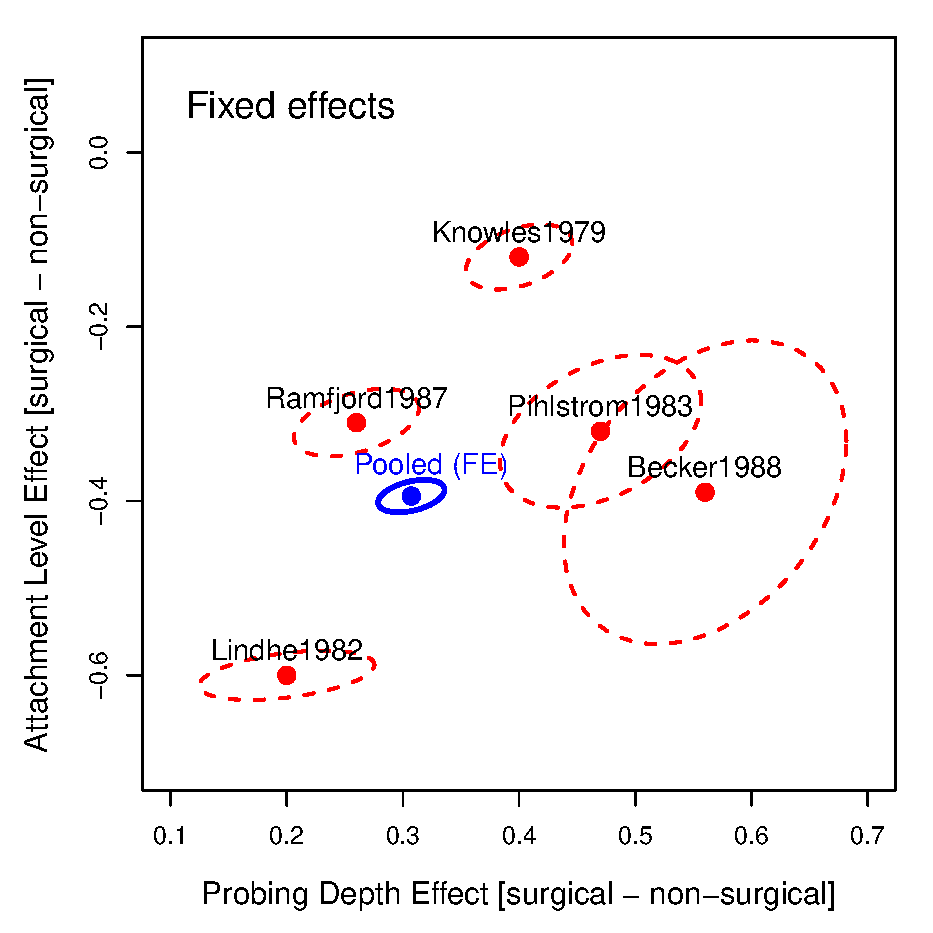
\includegraphics[width=1\linewidth]{fig/mvmeta2a}
%  \caption{}%
%  \label{fig:}
 \end{minipage}%
 \hfill
 \begin{minipage}[b]{.49\linewidth}
  \centering
  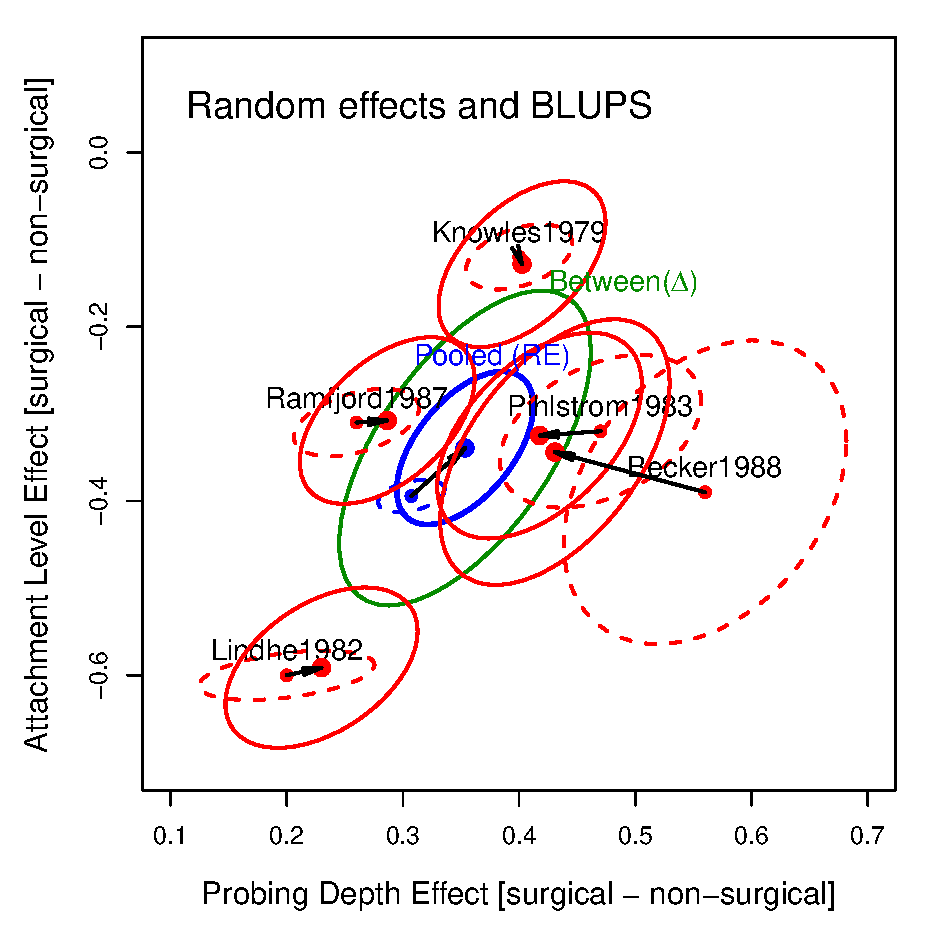
\includegraphics[width=1\linewidth]{fig/mvmeta2b}
 \end{minipage}
  \caption{Multivariate meta-analysis visualizations for five periodontal treatment studies with outcome measures PD and AL.
  Left: Individual study estimates $\vec{y}_i$ and 40\% standard ellipses for $\mat{S}_i$ (dashed, red) together with the pooled,
  fixed effects estimate and its associated covariance ellipse (blue).
  Right:  BLUPs from the random effects multivariate meta-analysis model and their associated covariance ellipses
  (red, solid), together with the pooled, population averaged estimate and its covariance ellipse (blue), and the estimate
  of the between-study covariance matrix, $\Delta$ (green). Arrows show the differences between the FE and the RE models.}
  \label{fig:mvmeta2}
\end{figure}

The left panel of \figref{fig:mvmeta2} shows the individual study estimates of PD and AL together with their covariances ellipses
in a generic form that we propose as a more useful visualization of multivariate meta-analysis results than standard
tabular displays: individual estimates plus model-based summary, all with associated covariance ellipsoids.%
\footnote{The analyses described here were carried out using the \texttt{mvmeta} package for R \citep{mvmeta}.}

It can be seen that all studies show that surgical treatment yields better probing depth (estimates are positive), while
non-surgical treatment results in better attachment level (all estimates are negative).  As well, within each study, there is a consistently
positive correlation between the two outcome effects: patients with a greater surgical vs.\ non-surgical difference on one
measure tend to have a greater such difference on the other, and greater within-study variation on PD than on AL.%
\footnote{Both PD and AL are measured on the same scale (mm), and the plots have been scaled to have unit aspect ratio,
justifying this comparison.}
The overall sizes of the ellipses largely reflect (inversely) the sample sizes in the various studies.
As far as we know, these results were not noted in previous analyses of these data.
Finally, the fixed-effect estimate, $\widehat{\vec{\beta}}^{\textrm{GLS}} = (0.307, -0.394)$,
and its covariance ellipse suggest that these effects are precisely estimated.

The random-effects model is more complex because $\vec{\beta}$ and $\mat{\Delta}$ must be estimated jointly.
A variety of methods have been proposed (full maximum likelihood, restricted maximum likelihood, method of
moments, Bayesian methods, etc.), whose details (for which see \citealp{Jackson-etal:2011}) are not relevant to the present discussion.
Given an estimate $\widehat{\Delta}$, however, the pooled, population-averaged point estimate of effects under the
random-effects model can be expressed as
\begin{equation} \label{eq:mvmeta5}
\widehat{\vec{\beta}}^{\textrm{RE}} = \left(\sum_i \mat{X}_i\trans  \mat{\Sigma}_i^{-1} \mat{X}_i  \right)^{-1}
                                      \left(\sum_i \mat{X}_i\trans  \mat{\Sigma}_i^{-1} \vec{y}_i \right) \comma
\end{equation}
where $\mat{\Sigma}_i = \mat{S}_i + \widehat{\mat{\Delta}}$.
The first term in \eqref{eq:mvmeta5} gives the estimated covariance matrix $\mat{V} \equiv \widehat{\Var}(\widehat{\vec{\beta}}^{\textrm{RE}})$
of the random-effect pooled estimates.
For the present example, this is shown in the right panel of \figref{fig:mvmeta2} as the blue ellipse.  The green ellipse shows the
estimate of the between-study covariance, $\widehat{\mat{\Delta}}$, whose shape indicates that studies with a larger estimate
of PD also tend to have a larger estimate of AL (with correlation = 0.61).
It is readily seen that, relative to
the fixed-effects estimate $\widehat{\vec{\beta}}^{\textrm{GLS}}$,
the unbiased estimate $\widehat{\vec{\beta}}^{\textrm{RE}} = (0.353, -0.339)$
under the random-effects model
has been shifted toward the centroid of the individual study estimates
and that its covariance ellipse is now considerably larger, reflecting between-study heterogeneity.
In contrast to the fixed-effect estimates, inferences on $H_0 : \widehat{\vec{\beta}}^{\textrm{RE}} = \vec{0}$
pertain to the entire population of potential studies of these effects.

\figref{fig:mvmeta2} (right) also shows the best linear unbiased predictions of individual study estimates
and their associated covariance ellipses, superposed (purely for didactic purposes)
on the fixed-effects estimates to allow direct comparison.
For random-effects models, the BLUPs have the form
\begin{equation} \label{eq:mvmeta6}
\widehat{\vec{\beta}}_i^{\textrm{BLUP}} = \widehat{\vec{\beta}}^{\textrm{RE}} + \widehat{\mat{\Delta}}  \mat{\Sigma}_i^{-1} (\vec{y}_i - \widehat{\vec{\beta}}^{\textrm{RE}}) \comma
\end{equation}
with covariance matrices
\begin{equation} \label{eq:mvmeta7}
\widehat{\Var}(\widehat{\vec{\beta}}_i^{\textrm{BLUP}}) = \mat{V} + (\widehat{\mat{\Delta}} - \widehat{\mat{\Delta}}  \mat{\Sigma}_i^{-1} \widehat{\mat{\Delta}})
\period
\end{equation}


Algebraically, the BLUP outcome estimates in \eqref{eq:mvmeta6}
are thus a weighted average of the population-averaged estimates and the study-specific estimates,
with weights depending on the relative sizes of the within- and between-study covariance matrices $\mat{S}_i$ and $\mat{\Delta}$.
The point BLUPs borrow strength from  the assumption of an underlying multivariate distribution of study parameters with covariance matrix $\mat{\Delta}$, shrinking toward the mean inversely proportional to the within-study covariance.
Geometrically, these estimates may be described as occurring along the locus of osculation of the ellipses
$\mathcal{E}(\vec{y}_i, \mat{S}_i)$ and $\mathcal{E}(\widehat{\vec{\beta}}, \widehat{\mat{\Delta}})$.

Finally, the right panel of \figref{fig:mvmeta2} also shows the covariance ellipses of the BLUPs
from \eqref{eq:mvmeta6}. It is clear that their orientation is a blending of the correlations in
$\mat{V}$ and $\mat{S}_i$, and their size reflects the error in the average point estimates $\mat{V}$
and the error in the random deviation predicted for each study.
